\chapter{Implementation}
\label{chapter:implementation}

EDCAT was implemented by combining a modified grader software used together with A+, which is a distributed e-learning platform and course management system. Both software are built with Python and fulfil distinct functionality; A+ provides the infrastructure for managing the exercises and students' submissions, and the grader is used for defining the exercises for the course and can be used to grade them. A+ provides a web interface built with Django while the grader is managed entirely through command line directly on the server.

First the user interface and its functionality is discussed in Section~\ref{section:functionality} after which we present the details of technical implementation in Section~\ref{section:technical}.


\section{Functionality}
\label{section:functionality}

The core functionality of A+ provides the means for a student to view exercise instructions, to submit exercises, and to see any of their own previous submissions. Maximum and earned points as well as the number of used submissions and the submission deadlines are shown both on exercise pages and course's main page as seen in Figure~\ref{figure:main}.

For the teacher or a teaching assistant A+ allows viewing all submissions, which they can resubmit, leave feedback for or adjust the grading of. The functionalities restricted to the teacher include for example modifying course's validity period, granting teaching assistant rights, and creating and modifying exercises. The functionality related to course management is discussed in more detail in Section~\ref{section:technical}.

\begin{figure}[t]
	\begin{center}
		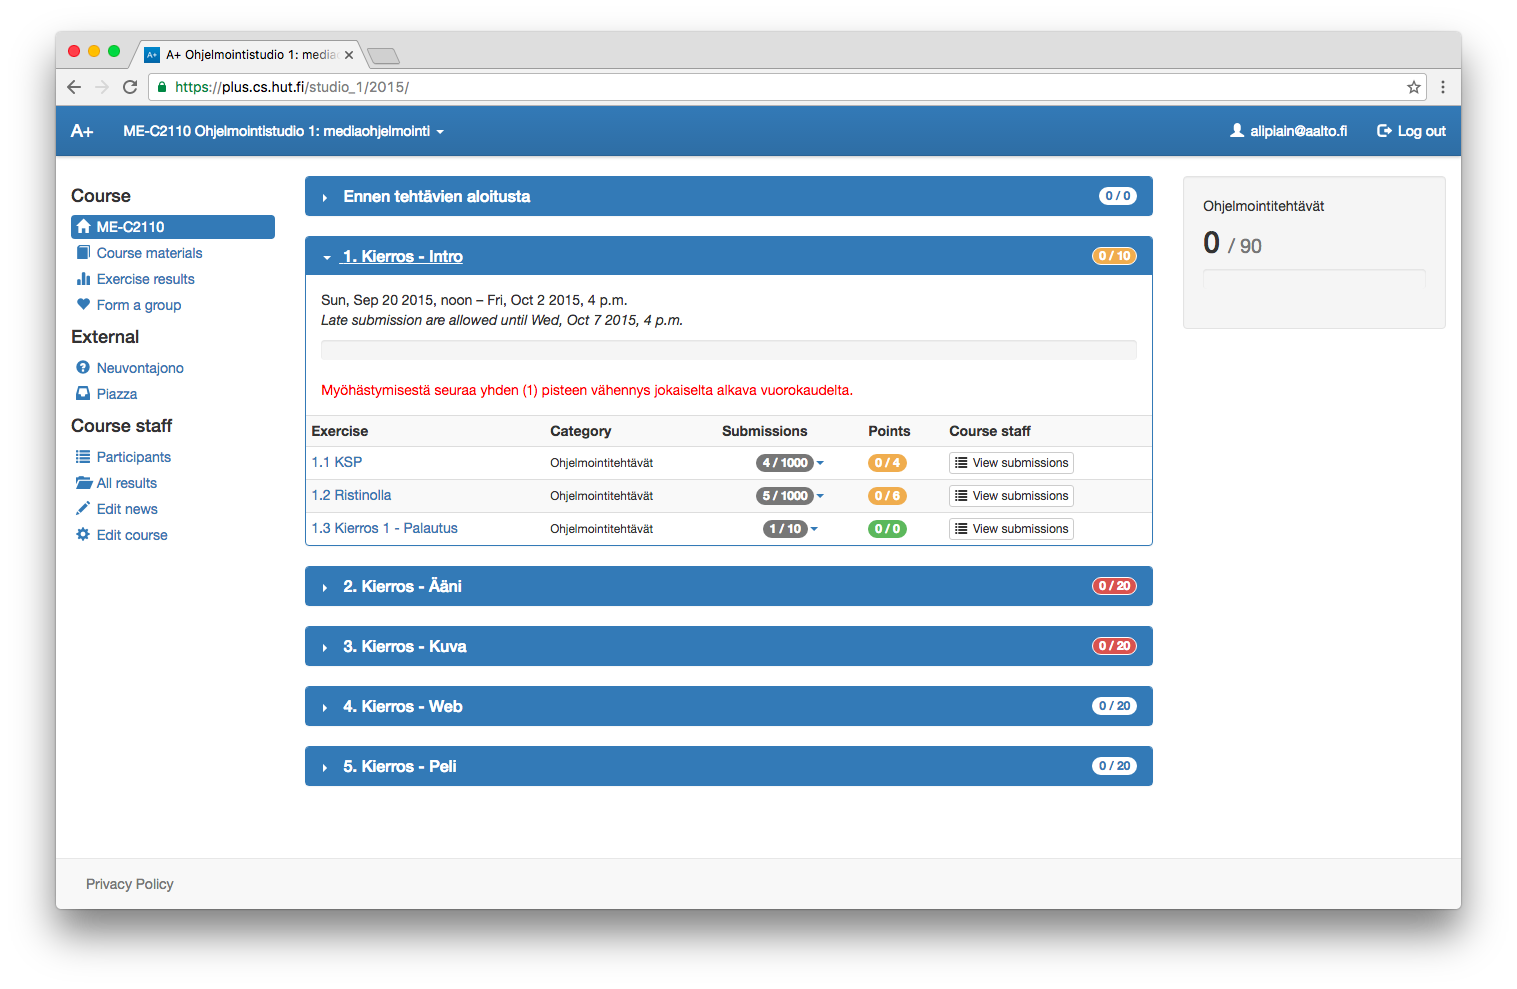
\includegraphics[width=\textwidth]{images/main.png}
	\end{center}
	\caption[asdf]{\small{The front page of a course with one module expanded. This screen capture was taken with the teacher privileges and shows links related to managing the course and submissions. The students are not able to see the content displayed under the \emph{Course staff} headings.}}
	\label{figure:main}
\end{figure}

The instruction pages function as submission forms for the exercises; at the bottom of each instruction page is a simple file upload form with fields for each required file. If the student tries to submit less than the number of required files, she is immediately redirected to the submission page with an error message that states that all files are required. If there is some problem with the submitted files, duplicate files or wrong files like for example \emph{.class} files, the submission results in a compilation error.

\begin{figure}[!ht]
	\begin{center}
		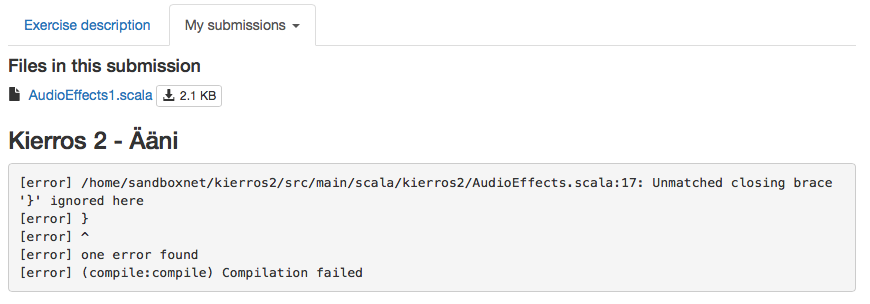
\includegraphics[width=\textwidth]{images/assignment_failed.png}
	\end{center}
	\caption[asdf]{\small{A detailed view of submission that resulted in a compilation error.}}
	\label{figure:failed}
\end{figure}

When the student successfully submits all the needed files, she is redirected to a submission page. If the grading of the submission takes some time, the student is presented with a progress bar and a message stating that the grading is taking longer than expected. The student is then required to wait and refresh the page in order to see the graded, or in this case compiled, submission. In case the compilation fails, the student is presented with a compilation error message similar to one in Figure~\ref{figure:failed}. If the submission compiles successfully, the resulting graphical user interface in JavaScript is presented. The graphical user interfaces used for this course are discussed in more detail in Section~\ref{subsection:GUIs}.


\subsection{Prepared Graphical User Interfaces}
\label{subsection:GUIs}

The graphical user interfaces used for the assignments, shown in Figures~\ref{figure:assignment1_1} through~\ref{figure:assignment3}, were relatively simple and easy to seamlessly embed to the base of the A+ system. The first assignment round consisted of two simple assignments --- the games of rock-paper-scissors and tic-tac-toe --- the GUIs to which are shown in Figures~\ref{figure:assignment1_1} and~\ref{figure:assignment1_2} respectively. The assignments familiarised students with random number generation and the basics of game programming.

\begin{figure}[!hb]
	\begin{center}
		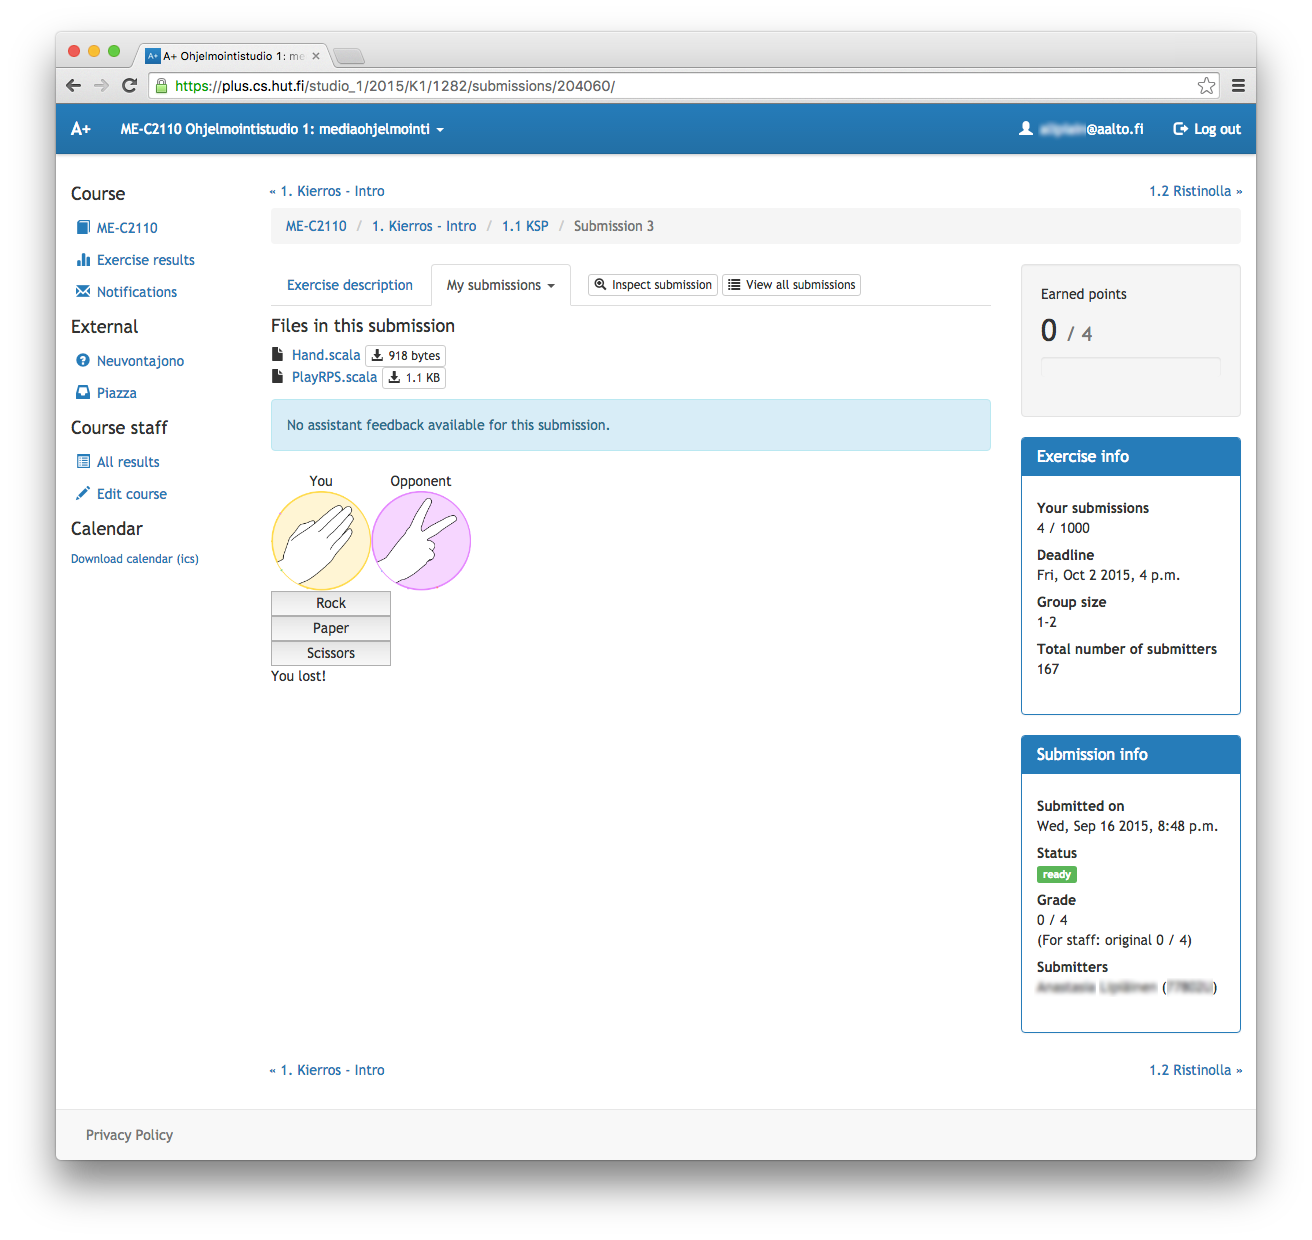
\includegraphics[width=\textwidth]{images/assignment1_1-mod.png}
	\end{center}
	\caption[asdf]{\small{The view of a successful submission to the assignment 1.1 with the resulting graphical user interface as JavaScript. The user has selected to play \emph{the paper} while computer opponent has randomly selected \emph{the scissors}. Below the buttons for the possible plays the user is shown the end result of the game -- in this case defeat.}}
	\label{figure:assignment1_1}
\end{figure}

The rock-paper-scissors GUI, pictured in Figure~\ref{figure:assignment1_1} in its basic form consist of three elements; an area to show both the user's and the computer selected hand, three buttons for selecting the hand to play, and an area to show the result of the game. The only interactive elements are the three buttons that all function alike. When the user selects a hand to play by pressing one of the buttons, the picture for user's hand is updated, the method that should return the computer's hand is called, picture for computer's hand is updated, and the end result of the game is updated.

\begin{figure}[!hb]
	\begin{center}
		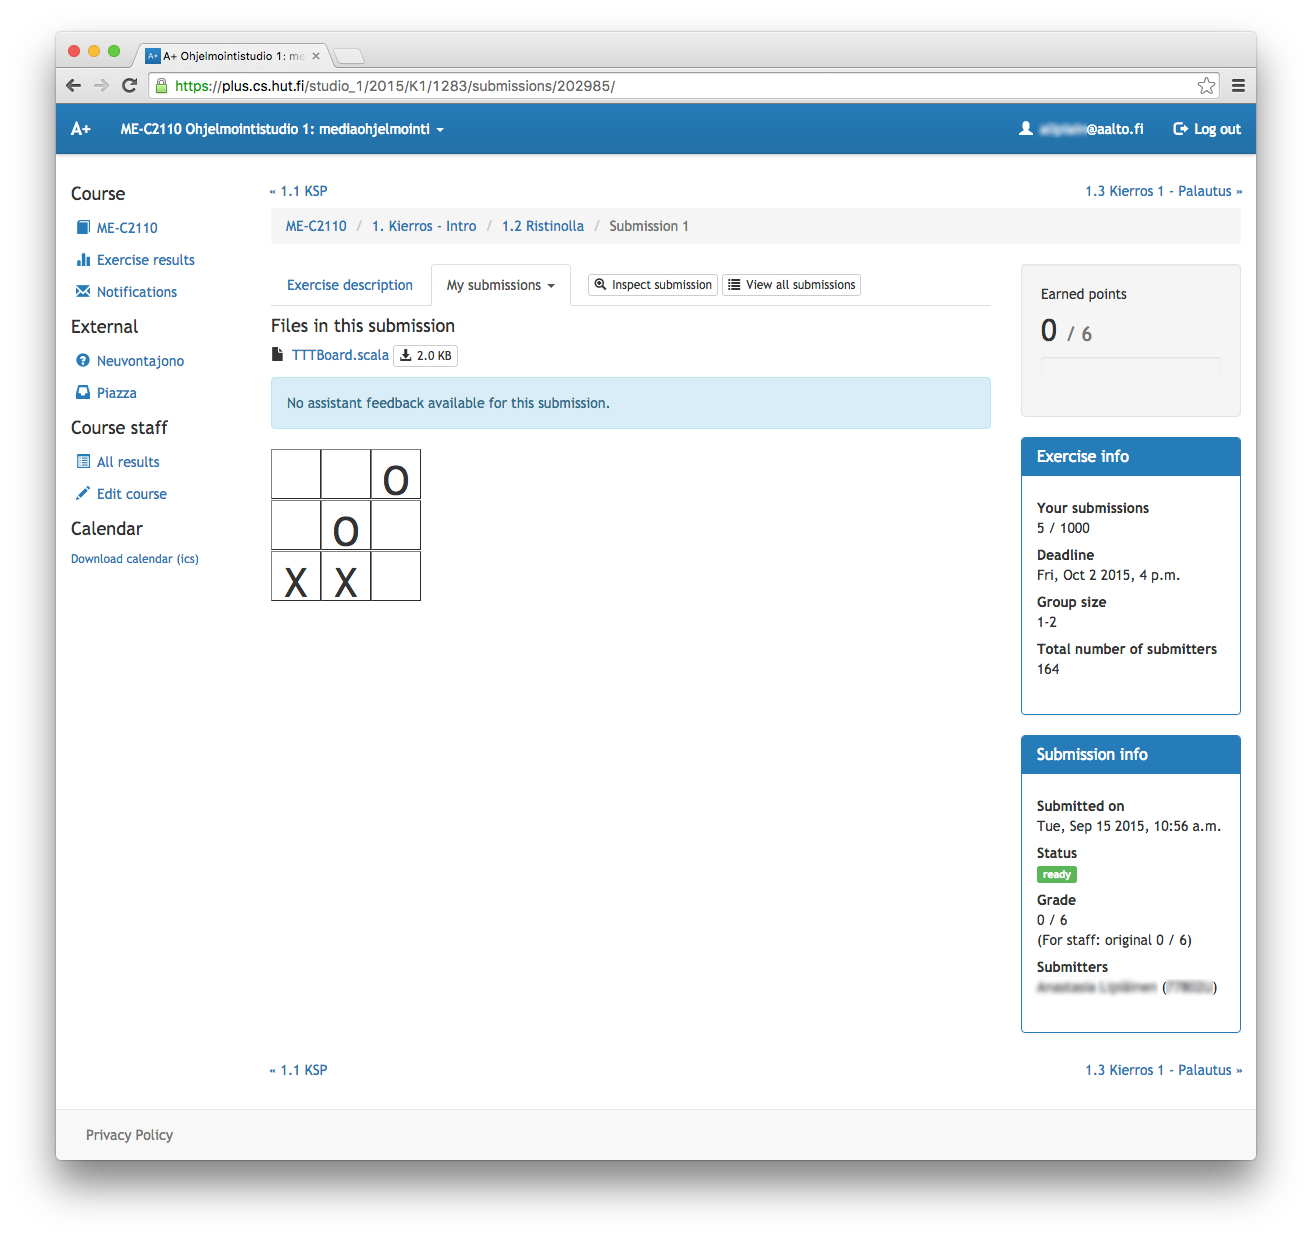
\includegraphics[width=\textwidth]{images/assignment1_2-mod.png}
	\end{center}
	\caption[asdf]{\small{The view of a successful submission to the assignment 1.2 with the resulting graphical user interface as JavaScript. The user plays the O marks while the computer opponent the X marks.}}
	\label{figure:assignment1_2}
\end{figure}

In order to carry out the assignment, the students are supplied with a project template that contains a skeleton for a Scala class to implement their solution to and a Scala class with a complete implementation of enumeration that models the possible plays of the game, in this case the hand gestures. For the students, the assignment is to implement the method that can randomly generate a hand for the computer player to play and the method that returns the end result of the game.

As a voluntary expansion on the mandatory work, the students were asked to extend the game with two additional plays of a lizard and Spock, which required adding some lines to the enumeration class and adjusting the logic in the method that returns the outcome of the game. The GUI was built so that it automatically generates buttons for all hands without requiring modifications to the GUI class.

The tic-tac-toe GUI, shown in Figure~\ref{figure:assignment1_2}, is even more simple than the rock-paper-scissors GUI. The grid of the game is build with nine buttons that show the played mark as text. When the game ends with either one of the players winning or every cell in the grid is filled, the end result of the game is showed beneath the game area similar to the rock-paper-scissors GUI.

The user gets to place the first mark by pressing the desired cell in the grid, which updates the text of the button to correspond to the user's mark. Then, until the game ends, the user and the computer get alternating turns. When it is the computer player's turn, the method that should return the coordinates of an empty cell to place the computer player's mark in is called. When the game ends, the method that returns the end result is called and the result is showed.

The student's assignment is to implement methods that allow querying and assigning a mark to the grid, which are used for drawing the grid and placing players' marks. Additionally, the student needs to implement methods that return truth-value for querying if the grid is full and if the game has ended, and most importantly the methods that return coordinates to place the computers mark in and the mark of the winner of the game. For the optional expansion students were asked to improve the AI of the computer opponent for which the required solution was to randomly return any of the empty cell coordinates. Similar to the first assignment, students were provided with the project template to implement their solution to. In the project template, there is a skeleton of a Scala class to implement the required methods to and an enumeration representing the marks, which allows successfully compiling the project locally.

\begin{figure}[!ht]
	\centering
	\small{
		\begin{subfigure}[The selected sound's waveform is shown at the top with all the interactive elements below.]{
			\centering
			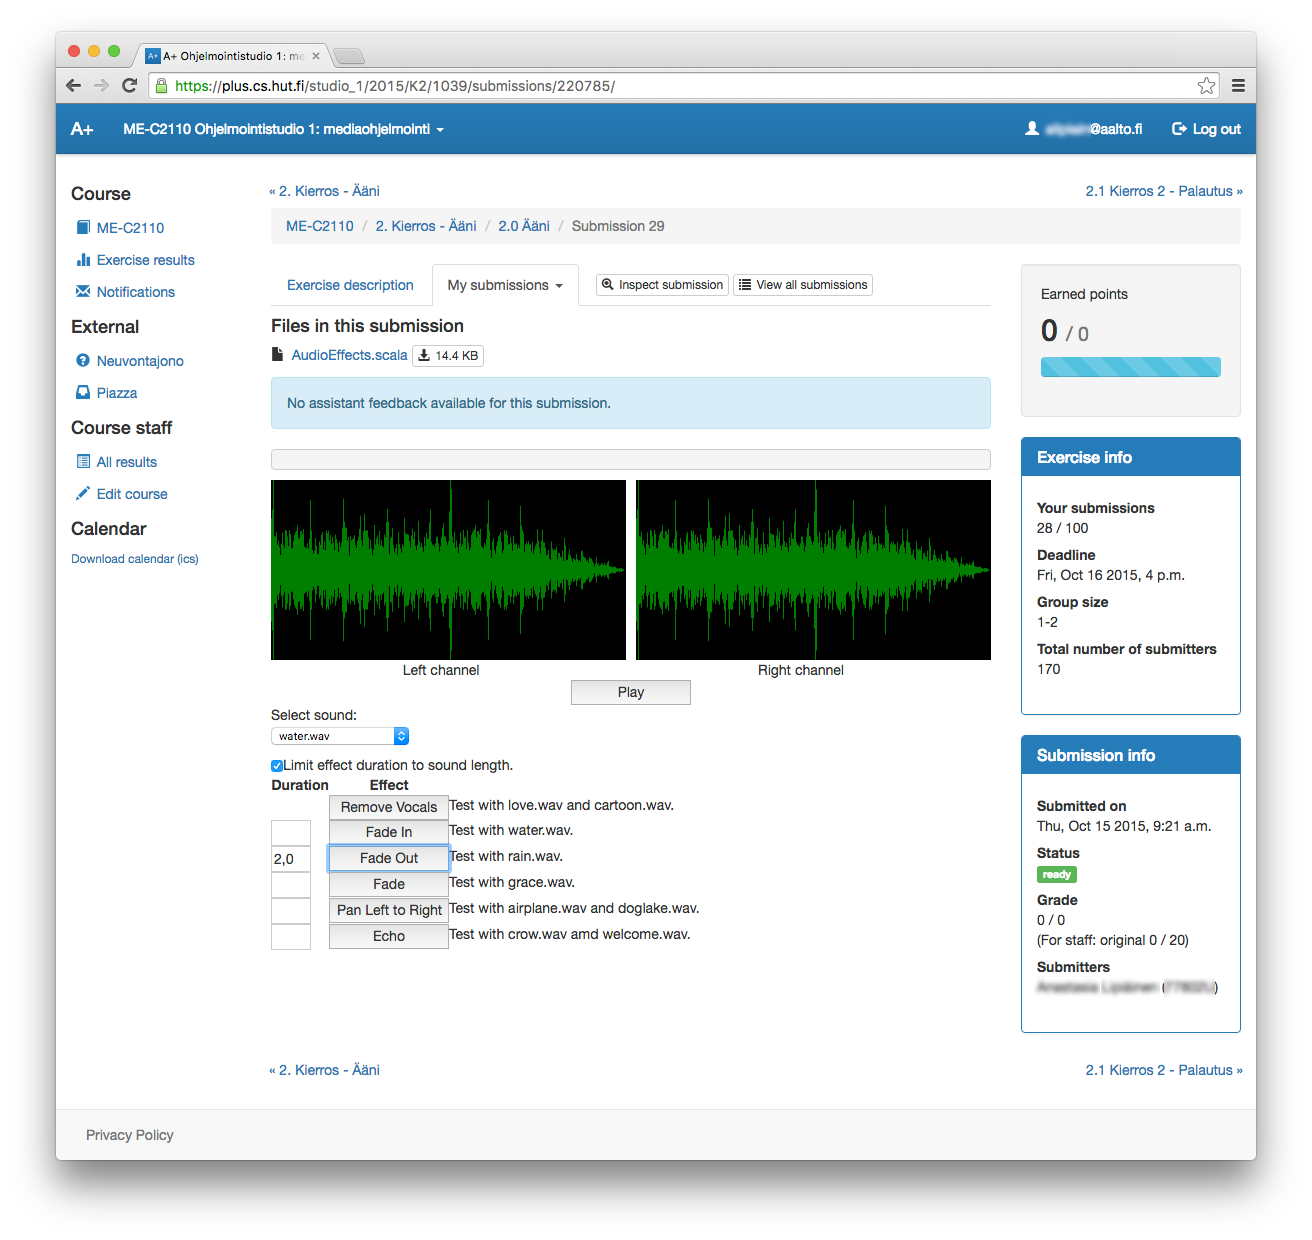
\includegraphics[width=\textwidth]{images/assignment2-mod.png}
		}
		\end{subfigure}
		\begin{subfigure}[An error message shown to the user after pressing the \emph{Echo} button without input to the accompanying field.]{
			\centering
			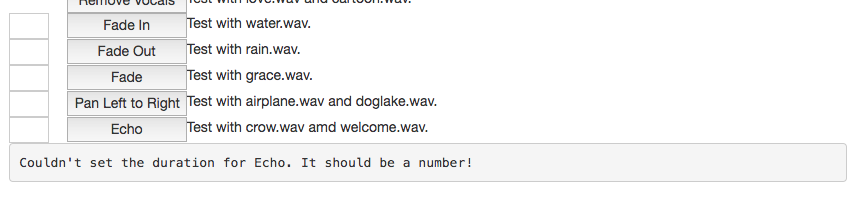
\includegraphics[width=\textwidth]{images/assignment2-failure.png}
		}
		\end{subfigure}
	}
	\caption{\small{The GUI in JavaScript with a highlight of an error message for the second assignment.}}
	\label{figure:assignment2}
\end{figure}

The solution for the second assignment round results in a sound manipulation program that uses student created filters to achieve various effects. The GUI, shown in Figure~\ref{figure:assignment2}, consists of four elements; the waveforms for the left and the right channels of the sound, a button to play the sound, the drop-down menu for selecting the sound, and the required input fields for using the implemented filters. The GUI is relatively static; the only updated elements are the waveforms and an error message is shown if the user inputs an invalid value to a field.

The waveforms are changed when the user selects a new sound or modifies the sound with a filter. The waveforms also feature an animated progress indicator, which is updated when the sound is playing. The error message, showcased in Figure~\ref{figure:assignment2}, is shown as preformatted text below the static UI. The input to the duration fields is expected to be given as seconds and allow only numerical input greater than zero with a comma as decimal mark. The fields can also be set to accept a value at most the length of the selected sound by selecting the checkbox marked \emph{Limit effect duration to sound length}. Submitting an invalid value will not have any side effects. Furthermore, when the user takes the use of field's spinners the value can be set to the precise value of sound's length.

\begin{figure}[!hb]
	\begin{center}
		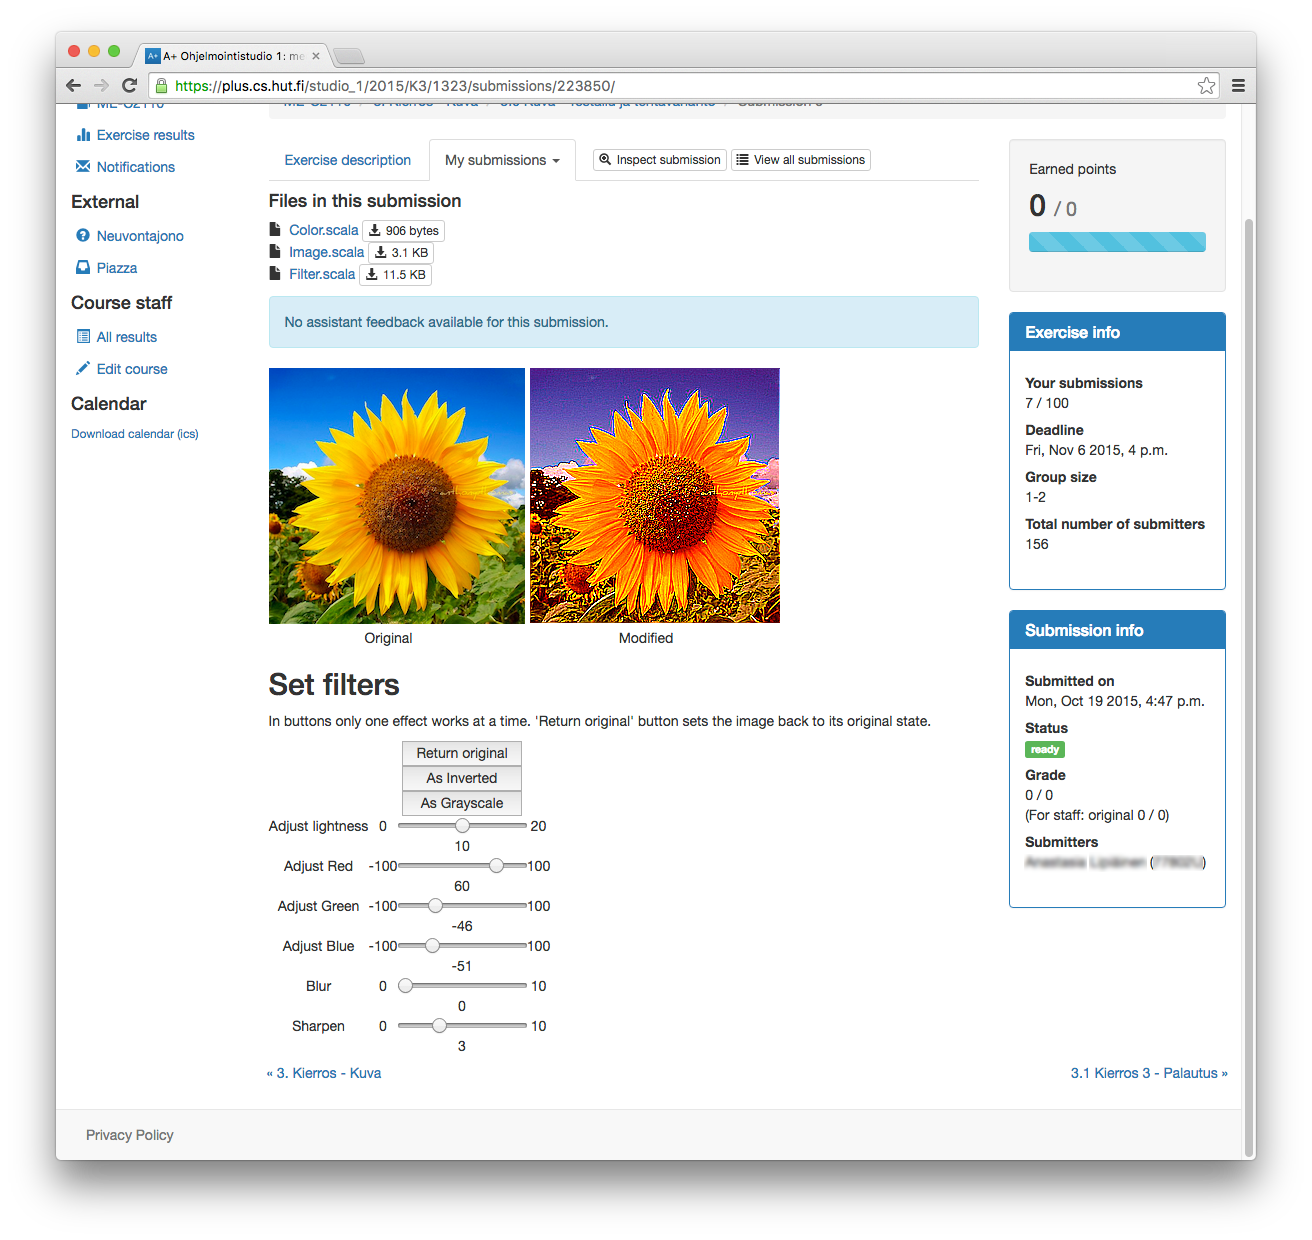
\includegraphics[width=\textwidth]{images/assignment3-mod.png}
	\end{center}
	\caption[asdf]{\small{The GUI in JavaScript returned for a successful submission to the third assignment. The image's colour and sharpness have been adjusted.}}
	\label{figure:assignment3}
\end{figure}

Pressing the \emph{Play} button causes the selected sound to be repeated. To keep things simple, there is no way to pause the playback and if the user presses the \emph{Play} button while a sound is playing, the repetition of the sound is started from the beginning while the previous playback is still played. Additionally, applying the filter not only modifies the sound but also repeats it.

Figure~\ref{figure:assignment2} shows all filters specified in the exercise instructions. The input fields and buttons are dynamically generated depending on the implemented functionality. In addition to the six required filters the students were welcome to implement any of their own that would be used either with only a button or a button and a numeric input field. The required filters included one that eliminates frequencies common to both the right and the left channels, four variation on a fading filter, and an echo filter. To facilitate the implementation, the students were again supplied with a project template attached with all the libraries required for a successful compilation.

The third assignment required students to create filters for image manipulation. The GUI is very similar to the sound manipulation GUI; the differences are that the image does not require a play button and is updated instantly, and the inputs to filters use buttons and sliders instead of number fields and buttons. The GUI in the third assignment did not have any dynamic error messages and is shown in its entirety in Figure~\ref{figure:assignment3}.

The GUI shows the original image always on the left while the modified image is updated on the right when the user applies the filters. The exercise instructions specify eight different image filters for students to implement. There are two filters that don't need any parameters and are applied using only a button --- those to invert the colours of the image and to convert the colours to greyscale. Additionally, there is a button that returns the modified image to its original state. The rest of the filters require input to adjust the intensity of the effect. There is a filter for adjusting the lightness of the image and three filters that adjust the colour components of the image in RGB colour space. Finally, the two more complex filters adjust the sharpness of the image.

As with the previous assignments, the students are provided with a project template to implement their solution into. This time they were required not only to implement the filters but also a class that models the colour in RGB colour space. For additional points, students could implement their own filters that could either take input from a slider or require no parameters.


\section{Technical Details}
\label{section:technical}

The exercises are created in A+ but they are managed through grader software. Furthermore, the actual code that defines the GUIs is written in Scala using Scala.js library. The following subsections explain in detail how the exercises are built and managed from the technical perspective.


\subsection{Course Management System}

The A+ system is hosted and developed by the \emph{Learning + Technology} group of Computer Science department in Aalto University. It is built with Python 3.7 and Django 1.7. and hosted on an Apache 2 server with uWSGI and Postgresql database. The maintenance team creates a course and an instance for the course and sets the teachers for the course, who have rights to fully manage the course. A teacher can set up the teaching assistants, but students can enrol to the course whilst it is visible by searching it through the landing page of the A+ system.

\begin{figure}[!ht]
\vspace{15px}
	\begin{center}
		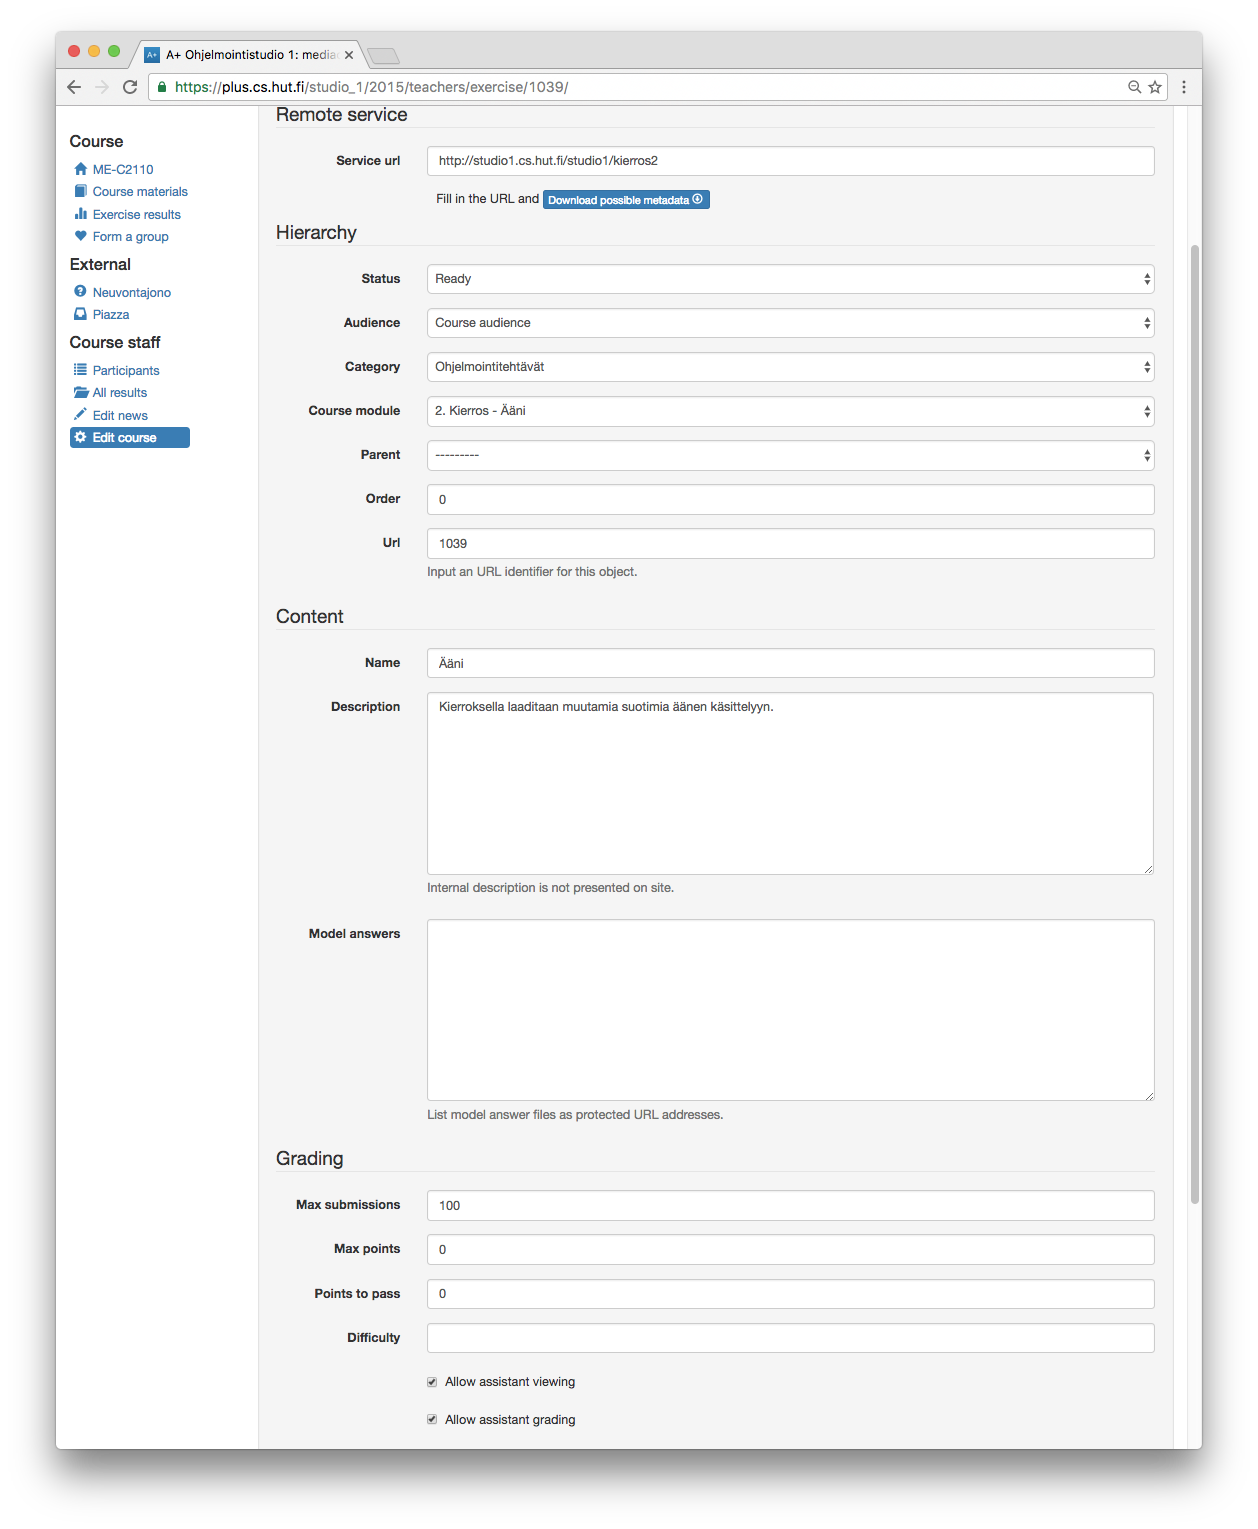
\includegraphics[width=\textwidth]{images/exercise-definition.png}
	\end{center}
	\caption[asdf]{\small{An example of the page to setup an exercise; here are shown the settings for the second assignment. Most of the information, like the exercise instructions, is fetched from service uri. The most important setting on A+ is the amount of maximum submissions.}}
	\label{figure:exercise-definition}
\end{figure}

The two most important features for the teacher of the course are creating exercises and viewing student's submissions. A course consists of modules that can contain one or several exercises as well as reading material. Modules have an opening and closing times, during which time all exercises in that module must be submitted unless late submission is allowed. There are four different kinds of exercise types available intended to be used with different grading methods and service models.

Our course had simple remotely hosted exercises that fetch the exercise definition from provided service URL. One example of an exercise definition is shown in Figure~\ref{figure:exercise-definition}. The service URL should point to a valid exercise definition file, whose structure is explained in Section~\ref{subsection:grader}. This exercise definition amongst other things has settings for the number of allowed submissions and points granted for the exercise. The number of allowed submissions was set so high that it was virtually limitless and students were not granted any points through the system, because grading was handled by the teaching assistants.

\begin{figure}[!b]
	\begin{center}
		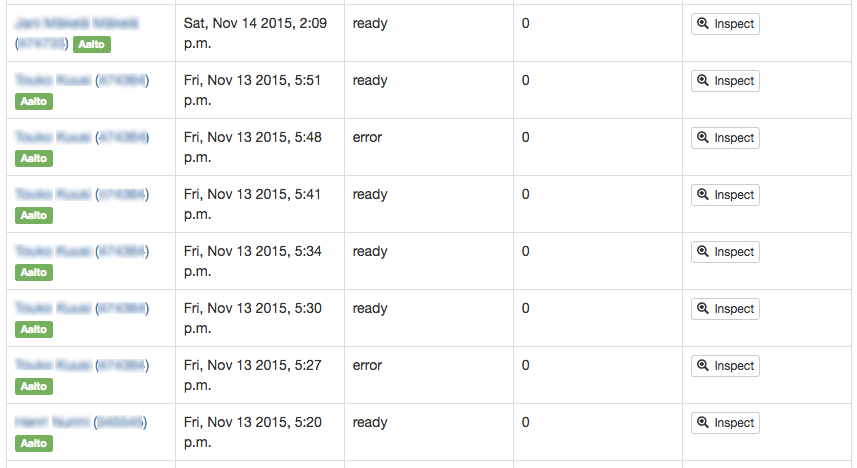
\includegraphics[width=\textwidth]{images/submissions-view-3-mod.png}
	\end{center}
	\caption[asdf]{\small{The excerpt from the submissions page with student names and numbers blurred. As visible, few of the assignments have resulted in a compilation error and their status is \emph{error}.}}
	\label{figure:submissions-view}
\end{figure}

The submissions are searchable and visible to both the teacher and the teaching assistants. You can see an excerpt from the submissions listing in Figure~\ref{figure:submissions-view}. The submissions can be searched with student's name or student number, submission date and result status. The submissions containing the submitted files and the feedback returned by the grading service can be individually inspected, as seen in Figure~\ref{figure:inspect-submission}. Additionally, both the teacher and the teaching assistants can leave feedback to the submission. This functionality was occasionally used by the teacher to interfere if a student had multiple consecutive erroneous submissions, and by teaching assistants to give verbal feedback for the assignment.

\begin{figure}[!t]
	\begin{center}
		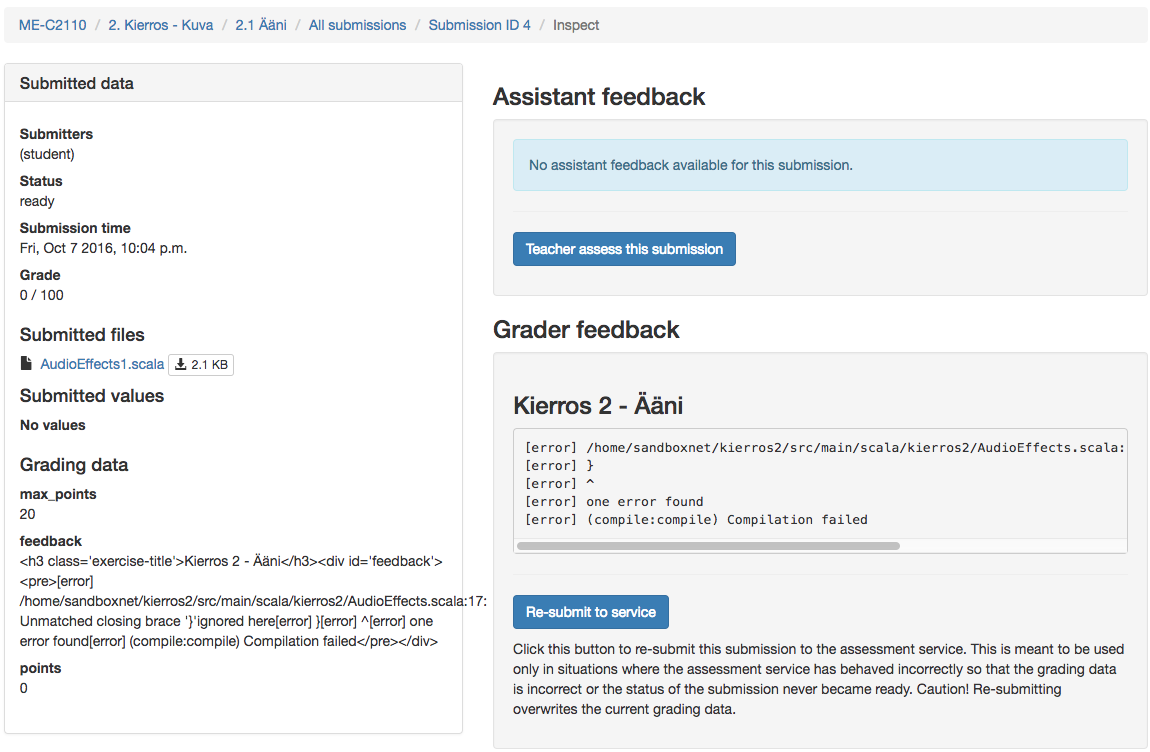
\includegraphics[width=\textwidth]{images/inspect-submission.png}
	\end{center}
	\caption[asdf]{\small{The excerpt from view for inspecting a submission. The teacher can also see the same view as the student by pressing the submission ID link. This page allows leaving feedback for the submission.}}
	\label{figure:inspect-submission}
\end{figure}


\subsection{Grader Software}
\label{subsection:grader}

The grader software was installed on a virtual server with Ubuntu 12.04.4 with 512MB of RAM and 10GB storage space. The grader is implemented using Django 1.7 with asynchronous grading queue using Celery 3.1, the grader works both with Python 2.7 and 3.4. The submissions are accepted via HTTP, graded in a sandboxed directory and discarded after grading. On top of standard requirements for grader software, the course required installing JDK 7, Scala 2.11.7 and sbt 0.13.7 for compiling the submissions.


\subsubsection*{Exercise Definition Files}

The course and its exercises are defined in subfolders with configuration files written in either JSON or YAML. The folder for the course contains an index file that defines the exercises as a list where each item or an exercise key must be pointed to a configuration file of the same name. In addition to the course list, the course configuration file contained definition for the name and the language of the course. All files related to the exercise, like additional program code or any other supporting files, are similarly stored in a folder that is named according to the exercise key.

%%%
% Define new float for listings
\newfloat{program}{b!}{lop}

% Define language for listing
\lstdefinelanguage{yaml} {
  morekeywords={title, description, instructions, view_type, files, field, name, max_points, actions, type, cmd,
								charset, expect_success, net, feedback_template},
  sensitive=true, % keywords are not case-sensitive
  morecomment=[l]{\#}, % l is for line comment
  morestring=[b]" % defines that strings are enclosed in double quotes
}

\definecolor{mymaroon}{HTML}{800000}

\lstset{
	caption={\small{The exercises are defined with YAML files that contain information shown to 
					 the students as well as information about what students should submit and how the 
					 submissions should be handled.}},
  abovecaptionskip=10pt,
	showlines=true,
	captionpos=b,label={listing:exerciseDef},
	language = yaml, alsoletter={.},
	numbers = left, numberstyle = \tiny,
	basicstyle = \scriptsize, showstringspaces = false,
	commentstyle = \color{blue}, keywordstyle = \color{mymaroon}
}
%%%

\begin{program}
\begin{lstlisting}
title: Exercise 1
description: The exercise results in a program.
instructions: | 
  <!-- Instructions for what students should do. HTML is a good
       option when the guidelines are complex or extensive -->

max_points: 0

# view_type field defines what is submitted.
# This definition states that students should submit
# two files named Main.scala and Helper.scala
view_type: access.types.stdasync.acceptFiles
  files:
    - field: file1
      name: Main.scala
    - field: file2
      name: Helper.scala

  actions: # What is done with the submission.
    - type: grader.actions.prepare
      charset: utf-8
    - type: grader.actions.sandbox
      cmd: [ "precompile.sh", "exercise_key", "Main Helper" ]
      expect_success: true
    - type: grader.actions.sandbox
      cmd: [ "sbt_compile.sh", "exercise_key", "Main Helper"]
      net: true
      expect_success: true
    - type: grader.actions.sandbox
      cmd: [ "assemble_submission.sh" ]

  # Passes raw grading task output.
  feedback_template: access/task_direct.html

\end{lstlisting}
\end{program}

All exercises for EDCAT were defined almost identically; each configuration file was similarly structured and the accompanying folders all contained build definition files for \emph{sbt}, the library files for Scala.js., Scala files containing the code needed for GUI, and the HTML file for the response GUI. The exercise configuration files were written in YAML and followed a similar structure of which you can see an example in Listing ~\ref{listing:exerciseDef}.

Of used attributes only \texttt{title} and \texttt{view\_type} were required. Each exercise definition file was additionally supplemented with \texttt{description}, \texttt{instructions}, and \texttt{max\_points} attributes. As the grader software was used together with A+, values of those additional attributes were directly relaid to the corresponding options of the exercise configuration inside the A+ system.

The \texttt{view\_type} attribute specifies the type of the exercise and especially how the exercise is submitted and graded. There are seven predefined types available, including different form and file submission options and it is also possible to define a specific \texttt{view\_type} for the course. In or course, all exercises were of type \texttt{acceptFiles}, which required students to submit one or more files that were then processed on the server and relaid to the asynchronous grading queue for compilation to JavaScript.

The \texttt{acceptFiles} type has itself both required and optional attributes that define what files should be submitted, how they are handled, and what is shown to the student. The configuration requires at least the list of expected files and the list of actions that will be performed on each submission. Additionally it is possible to specify the number of required files if not all are required, a message to show after the submission is accepted, whether the client should try to fetch the feedback automatically, and which templates are shown to the student for making the submission and as a response.

In addition to the required attributes of \texttt{acceptFiles}, our course utilised \texttt{feedback\_template} attribute, which specified to use a template that directly shows the feedback generated by actions. In our case, the feedback that actions generated was a HTML file embedded with the JavaScript compiled from submitted Scala code or a stack trace of a failed compilation.

An example definition of the \texttt{files} attribute of \texttt{acceptFiles} type is shown in Listing~\ref{listing:exerciseDef} on lines thirteen through seventeen.For each file, definitions for the field and file names should be supplied, and optionally information whether the file is required for the submission, which defaults to \texttt{true}.

Action list uses specific types of actions, of which there are seven predefined available and which can be defined to fit course specific purposes. The predefined action types have their own set of attributes but there are also attributes common to all action types. The common attributes include override options for awarded and maximum points, title for the action, whether the output should be written as HTML in a template and options to set what should be done if the action fails. EDCAT used \texttt{expect\_success} attribute that will on failure set the grading state to \emph{Error} and return from executing the actions. In the case of our course, the compilation tasks should be successful in order to continue onto assembling the response HTML.

The actions are executed in the order specified by the defined list seen on lines nineteen through thirty in Listing~\ref{listing:exerciseDef}. Of the seven available action types only \texttt{prepare} and \texttt{sandbox} were needed, while other actions included those specific for Python and \texttt{git} submissions, those that should be ran with separate grader software, and an action for storing student's submission without any manipulations.

The \texttt{prepare} actions are performed outside sandbox environment usually before the actual grading procedures and include tasks related to modifying files to allow grading. Attributes for moving and copying files are available as well as those for unpacking or setting the character encoding for the submission files. The submissions in our course were all first converted to use UTF-8 character encoding as seen on the line twenty-one of Listing~\ref{listing:exerciseDef}.

The \texttt{sandbox} actions are performed after chroot under a restricted user in a sandbox environment so potentially malicious or malfunctioning code can be executed safely. The functions performed are given in a \texttt{cmd} attribute that contains in an array a command for the command line followed by the required parameters. Other available attributes include settings for network usage, as seen on line twenty-seven of Listing~\ref{listing:exerciseDef}, or limiting the time, memory, disk space, and file usage. 

The commands used in our course were all defined in scripts. In the first and second assignment rounds the submissions were first compiled to JavaScript and then included in result HTML to return to the submitter (see lines twenty-six and thirty of Listing~\ref{listing:exerciseDef}). For the third assignment round the pre-compilation script, as seen on line twenty-three of Listing~\ref{listing:exerciseDef}, was added to shorten the time spent on malformed submissions.


\subsubsection*{Compilation Scripts}

As a response to the submission, the \texttt{task\_direct} template is returned to the A+ system regardless of the success of the submission. The template includes any possible content of standard error stream produced by the compilation process as preformatted text at the beginning of feedback. The content of standard output stream is presented as is, which means that the feedback upon successful compilation can be printed directly to the standard output stream.

The compilation process took use of three scripts of which one was used only in the third assignment round. The \texttt{precompile} script was added after the second assignment round in order to speed up the compilation process. The script takes as a parameter the files submitted by a student and the folder that holds the GUI code. It then attempts to compile all program code files together using \texttt{fsc} and returns the result of the compilation as exit status, i.e. the information whether the compilation was successful or failed.

If the files do not compile and produce an error with the accompanying error message, the error message will be included in the feedback passed onto A+ system and further scripts are not executed. Precompilation ensures that submission contains valid Scala code and requires spending significantly less time on clearly erroneous submissions instead of compiling them directly with much more time consuming \texttt{fastOptJS}.

The \texttt{sbt\_compile} script works analogous to \texttt{precompile} script. First the files are copied to network enabled sandboxed directory that also contains the GUI code. The compilation is done using \texttt{fastOptJS} that produces the JavaScript used in the response to the student. Because every compilation is performed in this same networked sandboxed directory, the JavaScript file is then copied to the student's submission folder and the files produced by the compilation --- like \texttt{.sjsir} and \texttt{.class} files as well as the JavaScript file and its source map --- are deleted. If compilation fails, the error message is conveyed to the A+ system and the \texttt{assemble\_submission} script is not executed.

Finally, the resulting JavaScript code is embedded in a HTML page to be passed to the A+ system. The \texttt{assemble\_submission} script prints out between \texttt{html} tags the contents of the JavaScript and \texttt{index.html} file.


\subsection{Creating GUIs with Scala.js}

Most importantly, every GUI designed to be used as a part of an exercise needed to be separate from the program logic written by students. Secondly, the exercises and GUIs needed to be to some extent extendable with students' own functionality. The used methods were explicitly defined in the exercise instructions and in second and third assignment rounds, where students wrote methods for their own filters, the filters were passed to the GUI as an iterable collection with functions as values.

All GUIs except the one for the sound manipulation assignment consist of just one class. The GUI for the second assignment needs more complex functionality which was separated and packaged to its own library. The GUIs are basically Scala code; each written as singleton object that utilises Scala.js, scala-js-dom~\footnote{ \url{http://scala-js.github.io/scala-js-dom/},\\~\url{https://github.com/scala-js/scala-js-dom}} and ScalaTags~\footnote{ \url{http://www.lihaoyi.com/scalatags/},\\~\url{https://github.com/lihaoyi/scalatags}} libraries. The Scala.js library provides annotation \texttt{JSExport}, that marks the object and needed method to be callable from the HTML that the JavaScript is embedded to. ScalaTags library is used for creating the HTML elements of the GUI and scala-js-dom library for access to some additional HTML elements like AudioContext and CanvasRenderingContext2D. A mock-up of GUI class can be seen in Listing~\ref{listing:GUI}.

% "define" Scala
\lstdefinelanguage{scala}{
  morekeywords={abstract,case,catch,class,def,%
    do,else,extends,false,final,finally,%
    for,if,implicit,import,match,mixin,%
    new,null,object,override,package,%
    private,protected,requires,return,sealed,%
    super,this,throw,trait,true,try,%
    type,val,var,while,with,yield},
  sensitive=true,
  morecomment=[l]{//},
  morecomment=[n]{/*}{*/},
  morestring=[b]",
  morestring=[b]',
  morestring=[b]"""
}

\definecolor{keywordcolor}{HTML}{7F0055}
\definecolor{stringcolor}{HTML}{2A00FF}
\definecolor{commentcolor}{HTML}{3F7F5F}
\definecolor{annotation}{HTML}{DE00AC}
\definecolor{localval}{HTML}{5E5EFF}
\definecolor{localvar}{HTML}{FF5E5E}
\definecolor{globalval}{HTML}{0000C0}
\definecolor{number}{HTML}{C48CFF}

\lstset{
	caption={\small{An example of what a GUI class looks like. The object and method that are referenced from the HTML need to marked with \texttt{JSExport} annotation. Otherwise the implementation is typical Scala code.}},
	captionpos=b,label={listing:GUI},
	language = scala, alsoletter={.},
	numbers = left, numberstyle = \tiny,
	basicstyle = \scriptsize, showstringspaces = false,
	stringstyle= \color{stringcolor},
	commentstyle = \color{commentcolor}, keywordstyle = \color{keywordcolor}\bfseries,
	moredelim=[is][\textcolor{annotation}]{\%\%}{\%\%},
  moredelim=[is][\textcolor{localval}]{\&\&}{\&\&},
  moredelim=[is][\textcolor{localvar}]{\#\#}{\#\#},
  moredelim=[is][\textcolor{globalval}]{\*\*}{\*\*},
  moredelim=[is][\textcolor{number}]{++}{++}
}

\begin{program}
\begin{lstlisting}
package exercise

import scala.scalajs.js

import scalatags.JsDom.all._

import org.scalajs.dom
import org.scalajs.dom.html

@js.annotation.%%JSExport%%
object Main {
  
  @js.annotation.%%JSExport%%
  def main(target: html.Div): Unit = {

    // methods used for operational logic and GUI generation

    // an example of an button definition
    val &&button&& = **input**(
      **`type`** := "submit",
      **value** := "button text"
    }
    &&button&&.##onclick## = (e: dom.Event) => {
      // do something
      update()
    }

    def update() : Unit = {
      // Remove all elements and add them anew
      val &&children&& = target.childNodes
      for (&&child&& <- ++0++ until &&children&&.length) {
        target.removeChild(&&children&&.item(&&child&&))
      }
      target.appendChild(
        **div**(
          **someTag**(
            **attribute** := "something else",
            **numericAttribute** := ++999++
          ),
          **otherTag**("some content"),
          &&button&&
        ).render
      )
    }
    update()
  }
}
\end{lstlisting}
\end{program}
Structure of each GUI implementation was similar; the main object had a method that constructed the interface in HTML tags and defined functionality for user interaction. The interaction was achieved by defining an inner function that was called when the HTML elements needed to be updated. Each interactive input element defined functionality for click or update event; in addition to changing the inner state of that element the update function was called.

All assignments but one, the tic-tac-toe game, used image or sound resources that were hosted separately from both the course management and grading systems. This means that in order to use those resources successfully, we had to deal with cross-origin HTTP requests. The server hosting media files was configured to accept \texttt{GET} requests from all domains. For sound and image manipulation assignments the resources were fetched from HTML code. However, because the rock-paper-scissors game was extendable by adding more plays, the students needed to have access to image representation definitions. The additional images were hosted in the same place as the default ones, so it was quite easy to deduce where to find those pictures needed for the extension.
